\documentclass{beamer}
\usepackage[english]{layout}
\usepackage[utf8]{inputenc}
\usepackage[english]{babel}
\usepackage[T1]{fontenc}
\usepackage{amsmath, soul, color, multicol, type1cm, verbatim, latexsym, dsfont, float, listings}
\usepackage[official]{eurosym}
\usepackage{beamerthemesplit}
\usepackage{hyperref}
\usetheme{Frankfurt}
\usecolortheme{lily}
%\usefonttheme{structuresmallcapsserif}
\usefonttheme{professionalfonts}
\setbeamercovered{transparent}

%NeSI Colors <---------------------------------------------------------------------------------------
\usecolortheme[RGB={47, 68, 71}]{structure} 
\definecolor{nesidark}{HTML}{2F4447}
\definecolor{nesilight}{HTML}{CED9DF}
\definecolor{nesigrey}{gray}{0.7}
\definecolor{nesilightgrey}{gray}{0.98}
\definecolor{nesidarkgrey}{gray}{0.3}
\definecolor{nesiblue}{HTML}{2B9FC2}
\setbeamercolor{block title}{fg=black,bg=nesigrey}
\setbeamercolor{block body}{bg=nesilightgrey,fg=nesidarkgrey}
\setbeamercolor{block body alerted}{bg=white,fg=black}
\setbeamercolor{alerted text}{bg=white,fg=black}

%\setbeameroption{show notes}

\setbeamerfont{title}{size=\huge}
\frenchspacing
\hyphenation{NeSI}

\newenvironment{topcolumns}{\begin{columns}[t]}{\end{columns}}
\newcommand\BackgroundPicture[1]{%
\setbeamertemplate{background}{%
\parbox[c][\paperheight]{\paperwidth}{%
\vfill \hfill \includegraphics[height=0.9\paperheight]{#1}
\hfill \vfill
}}}

\setbeamertemplate{blocks}[default]%[shadow=false]
\useinnertheme{circles}
\setbeamertemplate{title page}[default][center,rounded=false,shadow=false]
%\setbeamertemplate{title page}[default][center, wd=60mm, colsep=-4bp,rounded=true]

% Fancy Footer Content    <-----------------------------------------------------------------------------
%\setbeamertemplate{footline}{
%   \unilogo
%   \dsglogo
%   \begin{beamercolorbox}[ht=4ex,leftskip=1.4cm,rightskip=.3cm]{author in head/foot}
%    \usebeamercolor{nesiblue}
%    \hrule
%    \vspace{0.1cm}
%    \insertdate \hfill \inserttitle \newline
%    \insertshortauthor \ - \insertshortinstitute \hfill \insertframenumber
%   \end{beamercolorbox}
%   \vspace*{0.1cm}
%} 
% Reference http://joerglenhard.wordpress.com/2011/08/04/beamer-customization-ii-footline-with-multiple-lines/
% http://joerglenhard.wordpress.com/tag/beamer/
% https://github.com/lenhard/ub-beamer


\title{Introduction to HPC Workshop}
%\subtitle{Computational Science team}
\author{Centre for eResearch \\(eresearch@nesi.org.nz)}
\date{}


\begin{document}

{
%\setbeamertemplate{background canvas}{
\includegraphics[height=0.99\paperheight]{NeSI_img/Slide00.png}} 
\begin{frame}[plain]
\vspace{1cm}
\titlepage
\end{frame}
}


%\BackgroundPicture{NeSI_img/SlideXX.png}
\begin{frame}
\frametitle{Outline}
\begin{multicols}{2}
   \tableofcontents
 \end{multicols}
 \end{frame}


%%%%%%%%%%%%%%%%%%%%%%%%%%%%%%%%%%%%%%%%%%%%%%%%%%%%%%%%%%%%%%%%%%%%%%%%%%%%%%%%%%%%%%%%%%%%%%%
%%%%%%%%%%%%%%%%%%%%%%%%%%%%%%%%%%%%%%%%%%%%%%%%%%%%%%%%%%%%%%%%%%%%%%%%%%%%%%%%%%%%%%%%%%%%%%%

\section{About Us}
\frame[t]
{
  \frametitle{About Us}
     \begin{block}{CeR: Centre for eResearch}
   \begin{itemize}%[<+-| alert@+>]
	\item Part of the University of Auckland
	\item User support and system maintenance 
   \end{itemize}
  \end{block}
   \begin{block}{NeSI : New Zealand eScience Infrastructure}
   \begin{itemize}%[<+-| alert@+>]
	\item \textbf{NeSI} provides
	\begin{itemize}
		\item high performance computing
		\item a national data storage and sharing service 
		\item expert support and knowledge sharing 
		\item single-sign on across the NZ research sector
	\end{itemize}
   \end{itemize}
  \end{block}
}

\frame[t]
{
  \frametitle{About Us}
\begin{center}
\vspace*{1cm}
 
\includegraphics[width=150pt]{NeSI_img/nesi_logo.jpg}\\
 
\includegraphics[width=70pt]{NeSI_img/logo-u-of-a.jpg}
 
\includegraphics[width=70pt]{NeSI_img/logo-u-of-c.jpg}
 
\includegraphics[width=70pt]{NeSI_img/logo-niwa.jpg}\\
 
\includegraphics[width=70pt]{NeSI_img/logo-ministry-of-si.jpg} 
 
\includegraphics[width=70pt]{NeSI_img/logo-manaaki-whenua.jpg}
 
\includegraphics[width=70pt]{NeSI_img/logo-u-of-o.jpg}
\end{center}
}

\frame[t]
{
  \frametitle{About Us}
      \begin{block}{Our Team}
   \begin{itemize}%[<+-| alert@+>]
	\item We support researchers to get the most out of our platforms and services.
	\item As a team, we have a lot of experience in HPC that spans many science domains.
	\item Collaboratively enhance the performance of research software codes.
   \begin{itemize}
   	\item Troubleshoot memory and other or I/O bottlenecks.
	\item Connect researchers and scientific software experts.
	\item The team is available to support researchers across any research institution in New Zealand.
   \end{itemize}
   \end{itemize}
  \end{block}
}

\frame[t]
{
  \frametitle{About Us}
      \begin{block}{Support}
   \begin{itemize}%[<+-| alert@+>]
	\item Email \url{eresearch@nesi.org.nz}
	\item Creates a support ‘ticket’ where we can track the history of your request
	\item You can also arrange to meet us to discuss any issues
   \end{itemize}
   \begin{center}
   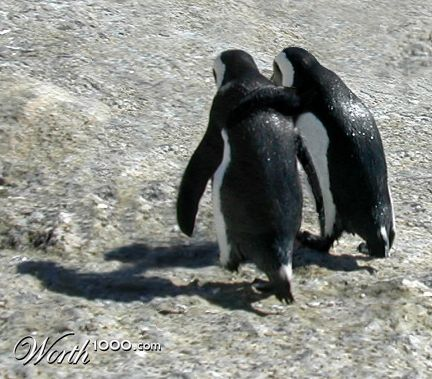
\includegraphics[width=100pt]{NeSI_img/pingu-friend.jpg}
   \end{center}
  \end{block}
}




\section{Key Concepts}
\frame[t]
{
  \frametitle{Key Concepts}
  \begin{columns}[onlytextwidth]
   
  \begin{column}{0.6\textwidth}
  
	  \begin{block}{What is a cluster}
      \begin{itemize}%[<+-| alert@+>]
	    \item A cluster is a network of computers, sometimes called nodes or hosts.
	    \item Each node has several CPUs (or cores). 
	    \item A CPU does the computing.
	    \item If your application uses more than one CPU, it can run faster on our cluster.
      \end{itemize}
      \end{block}
      \end{column}
      \begin{column}{0.4\textwidth}
      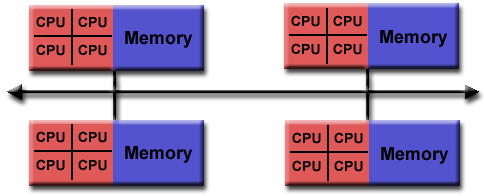
\includegraphics[width=140pt]{NeSI_img/hybrid_mem.png}
      \end{column}
   \end{columns}
}

% \note{Can the content of the node be changed by the image of the cpu's and the shared memory of a couple of slides further?}
% \frame[t]
% {
%   \frametitle{Key Concepts}
%    \begin{block}{HPC node overview}
%    \begin{center}
%  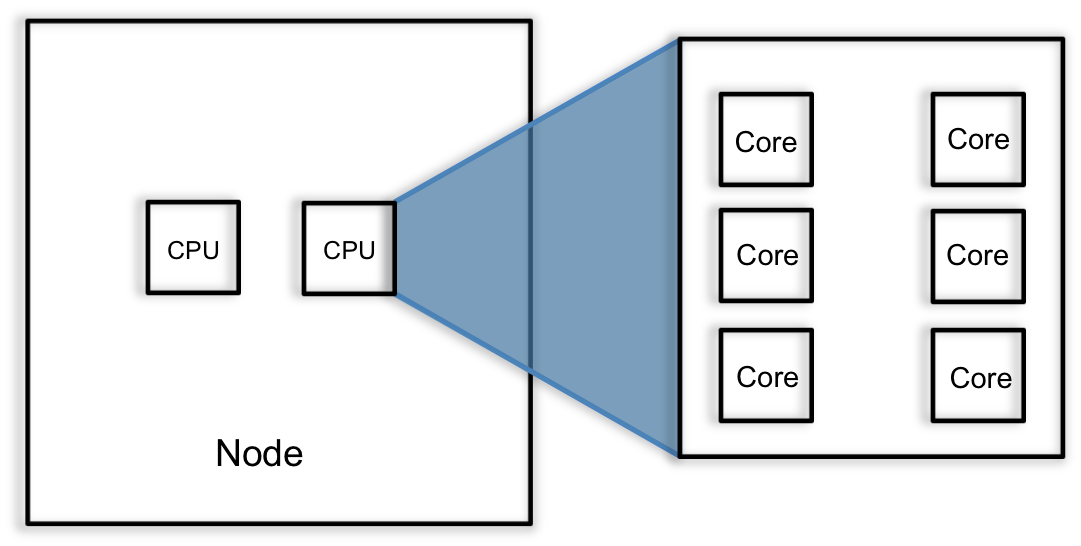
\includegraphics[width=270pt]{NeSI_img/node_view.png}
%    \end{center}
%   \end{block}
%   
% \begin{center}
% \end{center}
% }

\frame[t]
{
  \frametitle{Key Concepts}
      \begin{block}{Parallel Programming}
   \begin{itemize}%[<+-| alert@+>]
	\item There are several ways to make a program use more CPUs and hence run faster.
	\item Many scientific software applications are written to take advantage of multiple CPUs in some way. But often this must be specifically requested by the user at the time he runs the program, rather than happening automagically.
	\item We can help you improve the performance of your code or make better use of your application.
   \end{itemize}
  \end{block}
}

\frame[t]
{
  \frametitle{Key Concepts}
      \begin{block}{Shared Memory}
   \begin{itemize}%[<+-| alert@+>]
	\item Symmetric multiprocessing (SMP): two or more identical processors are connected to the same main memory.
	\item The program can divide tasks up between several threads. Each thread has access to all the program's data.
	\item There are different frameworks for utilizing SMP capabilities.
   \end{itemize}
\begin{center}
 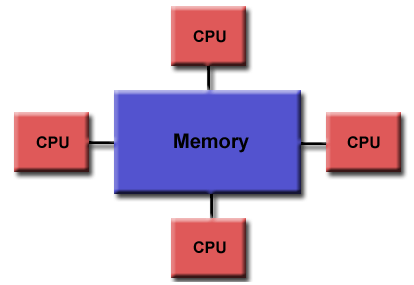
\includegraphics[width=90pt]{NeSI_img/shared_mem.png}
\end{center}
  \end{block}
}

%\frame[t]
%{
%  \frametitle{Key Concepts}
%      \begin{block}{Shared Memory : OpenMP}
%       \begin{itemize}%[<+-| alert@+>]
%	\item A master thread forks a specified number of slave threads and a task is divided among them. 
%	\item After the execution of the parallelized code, the threads join back into the master thread.
%	%\item Both task parallelism and data parallelism can be achieved using OpenMP in this way.
%   \end{itemize}
%\begin{center}
% \includegraphics[width=250pt]{NeSI_img/800px-Fork_join.png}
%\end{center}
%  \end{block}
%}


\frame[t]
{
  \frametitle{Key Concepts}
      \begin{block}{Distributed Memory}
   \begin{itemize}%[<+-| alert@+>]
	\item Multiple-processor computer system in which each process has its own private memory. 
	\item Computational tasks can only operate on local data.
	\item If remote data is required, the computational task must communicate with one or more remote processors.
	\item The most popular parallel programming paradigm is MPI (Message Passing Interface).
   \end{itemize}
\begin{center}
 %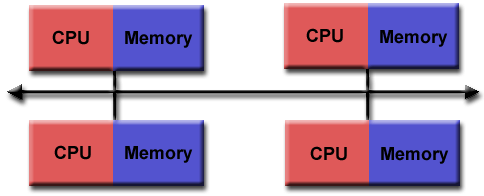
\includegraphics[width=120pt]{NeSI_img/parallel_paradigm/distributed_mem.png}
 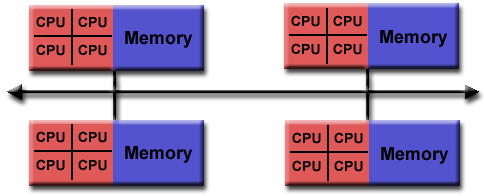
\includegraphics[width=150pt]{NeSI_img/hybrid_mem.png}
\end{center}
  \end{block}
}


\section{Our Facilities}
\frame[t]
{
  \frametitle{Our Facilities}
      \begin{block}{NeSI Facilities}
   NeSI provides several HPC architectures and solutions to cater for various needs:
     \begin{itemize}
     	\item BlueGene/P
	    \item Power6 and Power7
   		\item Intel Westmere
		\item Intel SandyBridge
		\item Intel IvyBridge \vspace{0.5cm}
		\item Kepler and Fermi GPU servers
		\item Intel Xeon Phi Co-Processor
   \end{itemize}
  \end{block}
}
\frame[t]
{
  \frametitle{Our Facilities}
      \begin{block}{NeSI Facilities}
   \begin{itemize}%[<+-| alert@+>]
	\item Many (though not all) supported applications can run on multiple NeSI architectures.% but for some of them there are more suitable architecture.
	\item We can install and test an application on all supported NeSI architectures and find the most suitable environment for your case.
	\item See the NeSI website for facility specifications and application details.
   \end{itemize}
  \end{block}
}

\frame[t]
{
  \frametitle{Our Facilities}
      \begin{block}{Pan, the NeSI CeR Supercomputing Centre}
   \begin{itemize}%[<+-| alert@+>]
	\item Funded by the \textbf{University of Auckland}, \textbf{Landcare Research} and the \textbf{University of Otago} with co-investment from the NZ Government through \textbf{NeSI}.
	\item Currently have around 6000 Intel CPUs across about 400 hosts.
	\item About 50 TB of memory.
	\item Shared storage of 400 TB with a 40 Gbit/s InfiniBand network.
	\item Runs Red Hat Enterprise Linux 6.3 as the operating system.
   \end{itemize}
  \end{block}
}

\frame[t]
{
  \frametitle{Our Facilities}
      \begin{block}{NeSI Pan Cluster}
      \begin{center}
       \begin{small}
      \begin{tabular}{|c|c|c|c|c|}
      \hline 
      \textbf{Architecture} & \textbf{Westmere} & \textbf{SandyBridge} & \textbf{IvyBridge}& \textbf{LargeMem} \\ 
      \hline 
      Clock Speed & 2.8\,GHz & 2.7\,GHz& 2.7\,GHz & 2.4\,GHz \\ 
      \hline 
      CPUs/socket & 6 & 8 & 12 &10 \\ 
      \hline       
      CPUs/node & 12 & 16 & 24 &40 \\ 
      \hline 
      Mem/node & 96\,GB & 128\,GB &  128/256\,GB& 512\,GB \\ 
      \hline 
      \# nodes & 76 & 194 & 42 &4 \\ 
      \hline 
      \end{tabular} 
      \end{small}
      \end{center}
  \end{block}
  We also have GPUs and Intel Xeon Phi's available. More information on the documentation page under \textsl{Available hardware.}
}
\section{Using the Cluster}      

\frame[t]
{
  \frametitle{What to expect}
      \begin{block}{Suitable work}
   \begin{itemize}%[<+-| alert@+>]
	\item Problems that can be solved with parallel processing.
	\item Problems that consume large amounts of memory.
	\item Problems that render your desktop useless for long periods of time.
   \end{itemize}
  \end{block}
        \begin{block}{Less suited}
   \begin{itemize}%[<+-| alert@+>]
	\item Windows-only software $\mapsto$ Aspirational Research Virtual Machine Farm. 
	\item Interactive software, e.g.\ GUI, only available for development (in general).
   \end{itemize}
  \end{block}
}


\frame[t]
{
  \frametitle{What to expect}
      \begin{block}{Scaling behaviour}
   \begin{itemize}%[<+-| alert@+>]
	\item Some problems are ``embarrassingly parallel'', i.e.\, it is trivial to divide the problem and solve independently.\\For instance, you could run the same simulation with 1000 different initial conditions.
	\item Approximately linear speedup.
	\item Other problems have dependencies, they cannot be separated\\e.g. simulating the weather.
	\item Speedup depends what \% of the program runtime can be parallelised.
   \end{itemize}
  \end{block}
}


\frame[t]
{
\begin{topcolumns}
\column{0.5\textwidth}
    \begin{block}{Amdahl’s Law}
    \begin{center}
      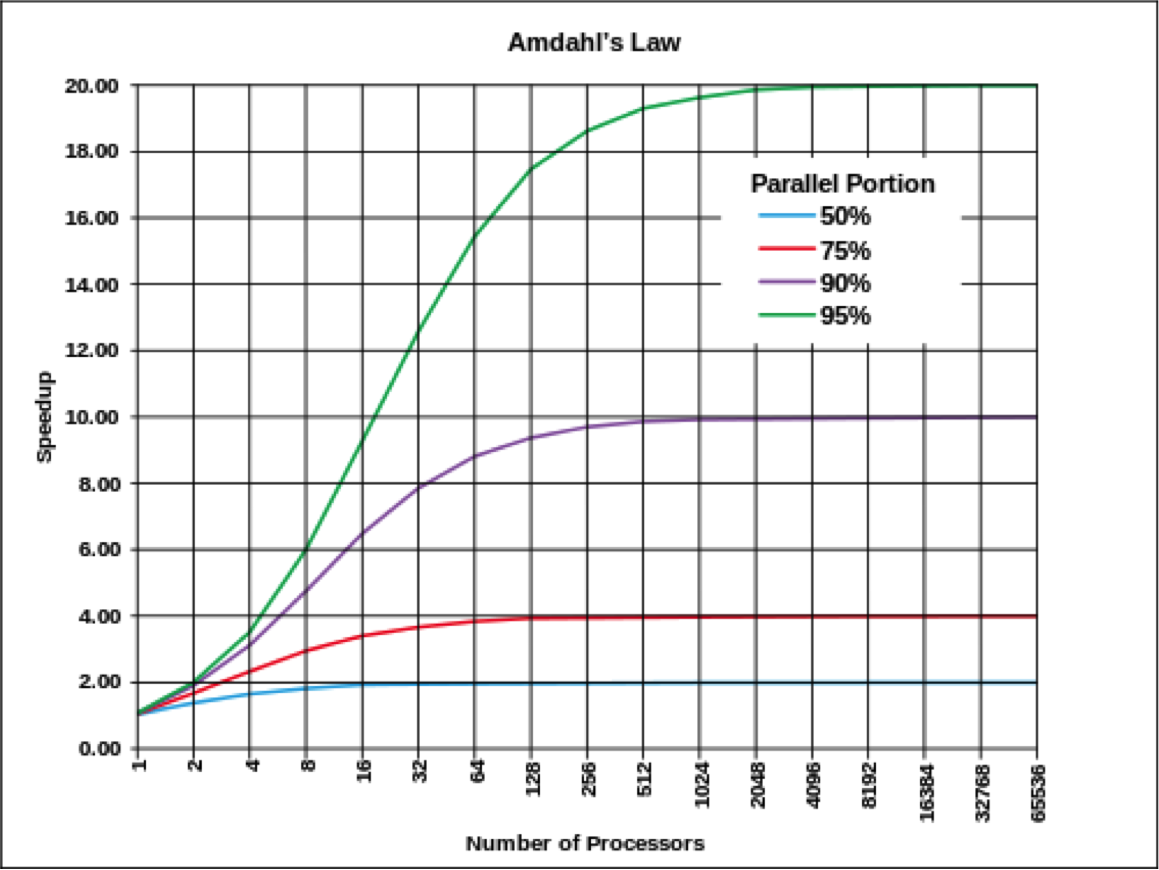
\includegraphics[width=120pt]{NeSI_img/Amdahl.png}
    \end{center}
    \end{block}
\column{0.5\textwidth}
     \begin{block}{Real Case: more CPUs $\neq$ more speed}
   \begin{center}
   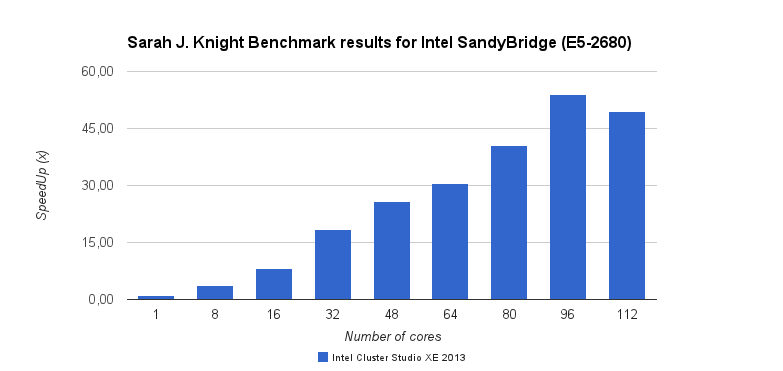
\includegraphics[width=160pt]{NeSI_img/migrate_scalability.png}
   \end{center}
  \end{block}
  \end{topcolumns}
}

\frame[t]
{
   \begin{block}{Parallel execution time}
   \begin{itemize}%[<+-| alert@+>]
	\item Single CPU computation time: computation only.
	\item Parallel computation time: computation + communication + waiting.
	\item For example:
	\begin{itemize}
	\item Writing results (to one file) is often a bottleneck.
	\item Small problem on many cores: communication costs will dominate.
	\item Unbalanced load: one slow CPU will hold up all the others.
	\end{itemize}
	\item Conclusion: Test which number of CPUs is best suited for your problem. 
   \end{itemize}
  \end{block}

}



\frame[t]
{
  \frametitle{General overview}
      \begin{block}{Using the cluster}
\begin{center}
 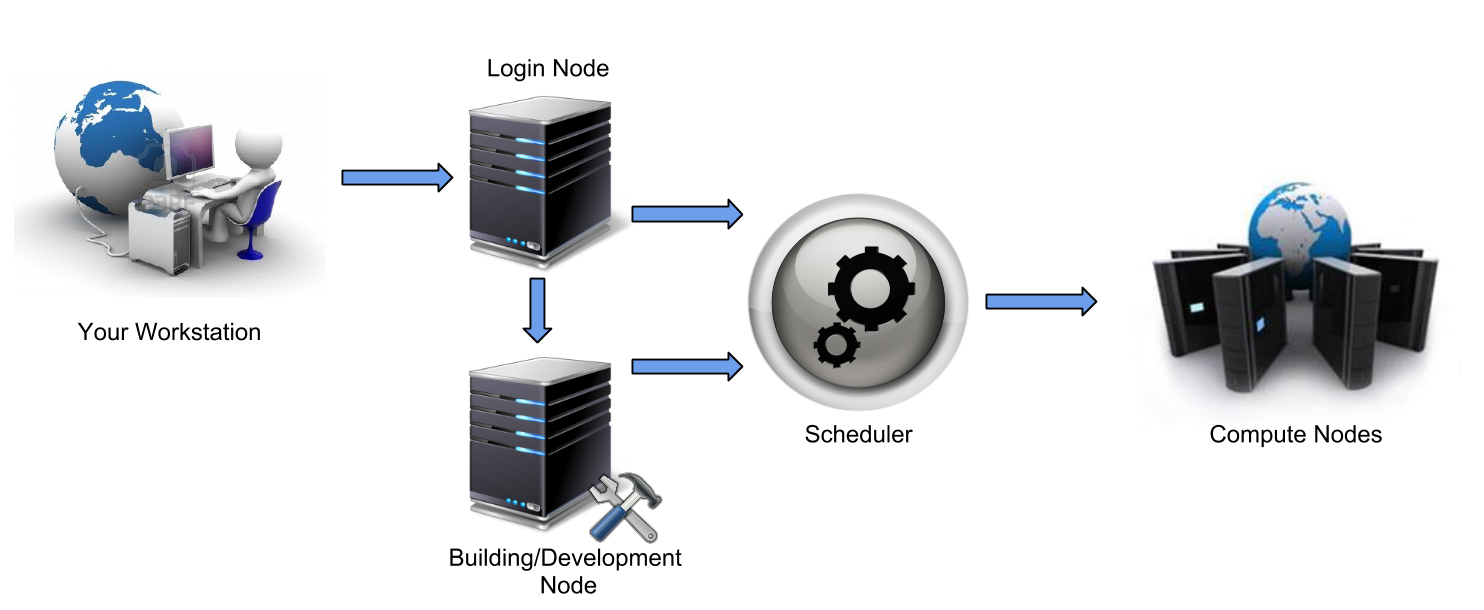
\includegraphics[width=310pt]{NeSI_img/NeSI_compute_path.png}
\end{center}
  \end{block}
}



\frame[t]
{
  \frametitle{Using the Cluster}
      \begin{block}{Overview}
   \begin{itemize}%[<+-| alert@+>]
	\item The cluster is a shared resource and work must be scheduled.% to run at a later time, known as batch scheduling – no GUI.
	\item Jobs are queued and are executed on the compute nodes.
	\item The login node is not for running jobs, it is only for file management and job submission.
   \end{itemize}
  \end{block}
  \begin{center}
 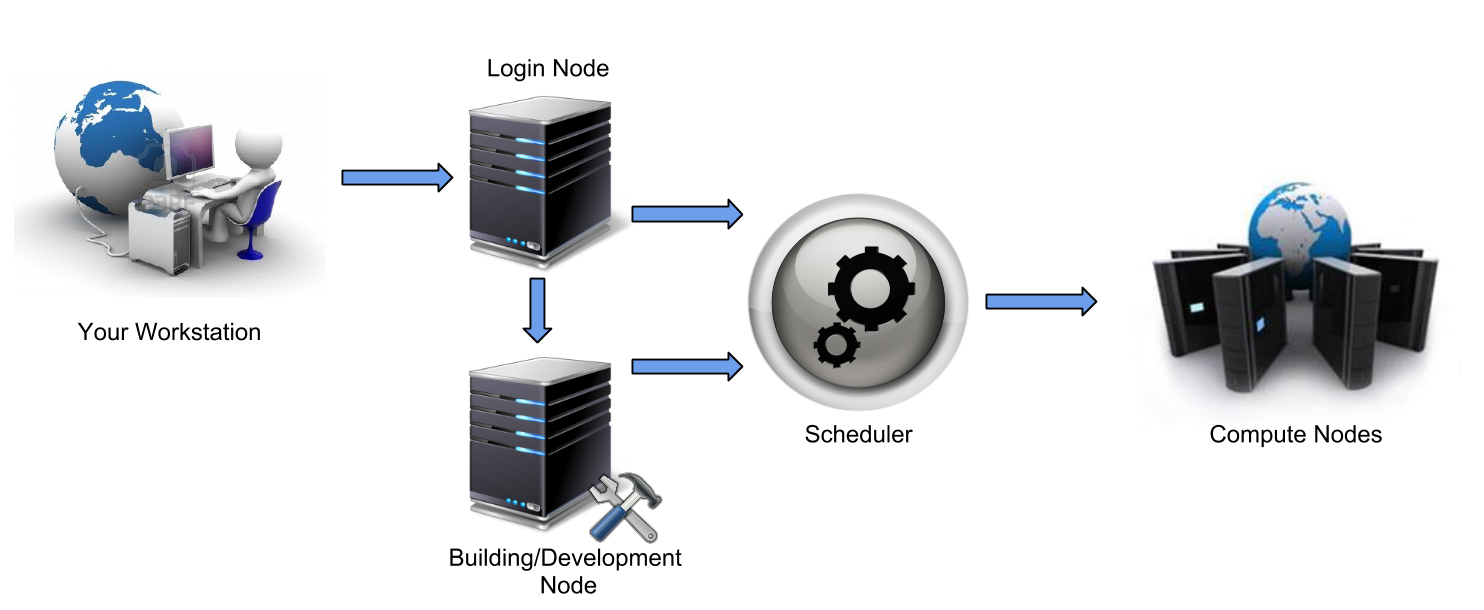
\includegraphics[width=200pt]{NeSI_img/NeSI_compute_path.png}
\end{center}
}
\frame[t]
{
  \frametitle{Using the Cluster}
      \begin{block}{Compiling and Testing Software}
   \begin{itemize}%[<+-| alert@+>]
	\item In each NeSI facility you will find building/development nodes.
	\item We have the most up-to-date development tools ready to use.
	\item You can build and test your software and then submit a job.
   \end{itemize}
  \end{block}
  \begin{center}
 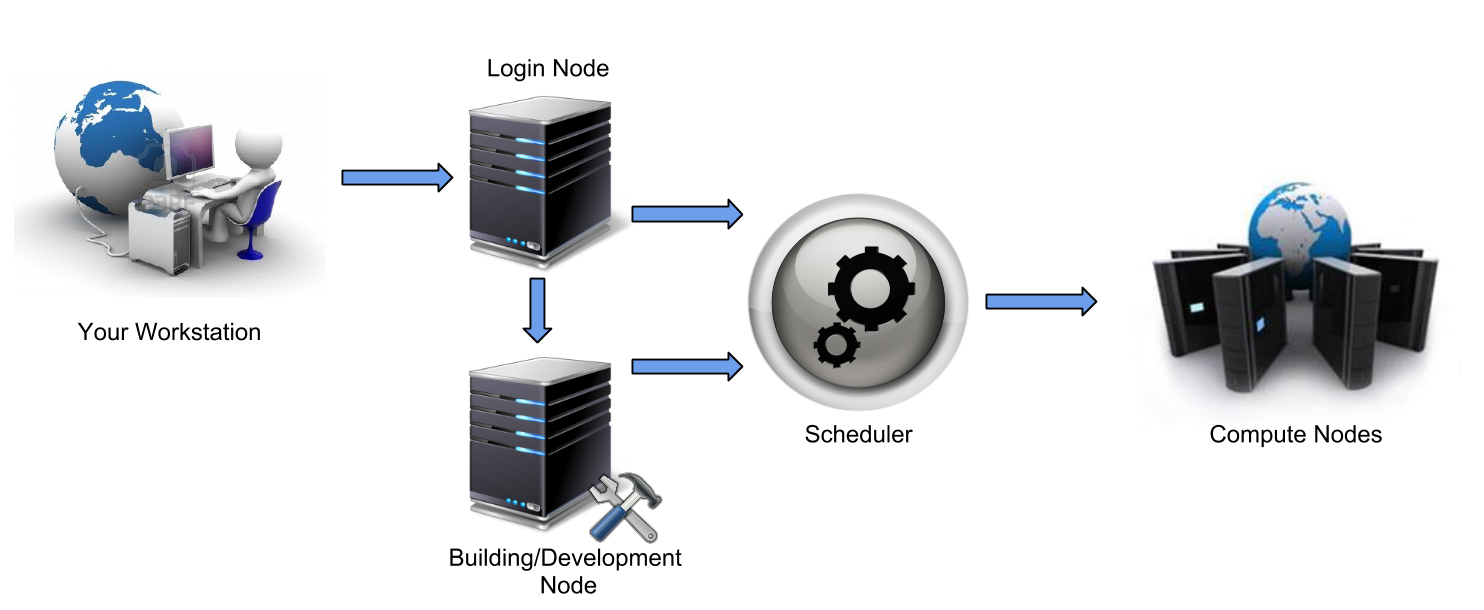
\includegraphics[width=200pt]{NeSI_img/NeSI_compute_path.png}
\end{center}
}


\frame[t]
{
  \frametitle{Using the Cluster}
      \begin{block}{Connection via SSH}
      There is software available for each desktop operating system that implements the Secure Shell (SSH) protocol:
        \begin{itemize}
        \item Windows: \href{http://mobaxterm.mobatek.net/}{MobaXterm} (third-party, not included with the OS)
        \item Mac OS X: Terminal (shipped with the OS), \href{http://www.iterm2.com/}{iTerm2} (third-party, not included)
        \item Linux: \href{http://konsole.kde.org/}{Konsole}, Gnome Terminal, \href{http://yakuake.kde.org/}{Yakuake}
        \end{itemize}
        Whichever terminal you use, you will need to run a command like:\\ssh \url{jbon007@login.uoa.nesi.org.nz}
      \end{block}
}





\begin{frame}[fragile]
  \frametitle{Using the Cluster}
      \begin{block}{Remote File System Access}
       In order to access the file system (/home) remotely from your machine, we recommend:
        \begin{itemize}
        \item \textbf{Windows} (mobaxterm): \href{http://mobaxterm.mobatek.net/}{mobaxterm}
        \item \textbf{MacOSX} (SSHFS): \url{http://code.google.com/p/macfuse/}
        \item \textbf{Linux} (SSHFS): \url{http://fuse.sourceforge.net/sshfs.html}
        \item \textbf{Linux} (scp): \url{https://linuxacademy.com/blog/linux/ssh-and-scp-howto-tips-tricks/}
        \item \textbf{KDE} (Konqueror): type fish://user@host:port
        \item \textbf{Gnome} (Nautilus): type sftp://user@host:port
      \end{itemize}
      \end{block}
\end{frame}



\frame[t]
{
  \frametitle{Using the Cluster}
      \begin{block}{Data}
   \begin{itemize}%[<+-| alert@+>]
	\item Upload input data to the login node for use on the cluster.
	\item Download results from the login node to your local drive. 
	\item Your home directory has a small quota. Project directories are significantly larger.
	\item Things do go wrong. Keep your own backups of anything important.
	\item For long-term storage and backups, consult your institution's IT department.
	\item Files on the login node are shared across the build and compute nodes.
   \end{itemize}
%   \begin{center}
%   
\includegraphics[width=125pt]{NeSI_img/kami23-doubtux.png}
%   \end{center}
  \end{block}
}

\section{Submitting a Job}


\frame[t]
{
  \frametitle{Submitting a Job}
      \begin{block}{Basic Job Properties}
   \begin{itemize}%[<+-| alert@+>]
	\item \textbf{Name}: For easily identifying the job (in the queue) and its output files.
	%\item \textbf{Command} What command to execute on the cluster e.g "echo hello"
	\item \textbf{Walltime}: How long can the job run for? The job will be killed if it runs out of time. 
	\item \textbf{Memory}: How much to use? The job will die if it needs more memory than you allow.
	\item \textbf{CPUs}: How many to use? Some programs try to use more CPUs than they are allocated, e.g.\ MATLAB.
	%\item \textbf{Files} You need to specify where additional files can be found and change references in your scripts
	\item \textbf{Account information}: Especially important for access to funded research allocations
	\item \textbf{Emails}: Whom, and in what circumstances, the scheduler will notify about changes to the job status.
   \end{itemize}
  \end{block}
}


\frame[t]
{
  \frametitle{Submitting a Job}
      \begin{block}{Outputs}
   \begin{center}
   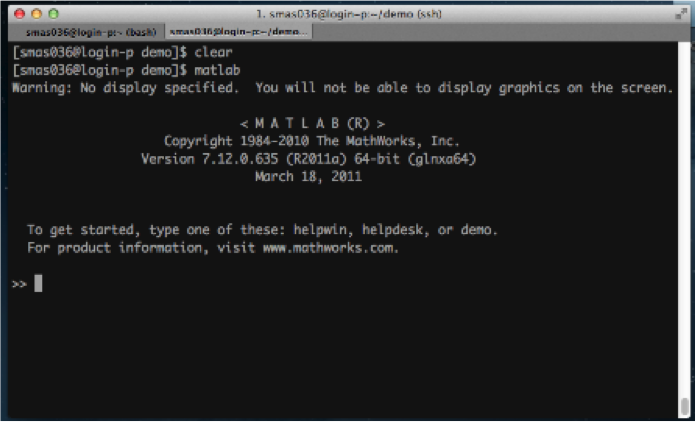
\includegraphics[width=200pt]{NeSI_img/console.png}\\
      Jobs have no interactive interface, but write to files. Text written to the command line output and error channels will also be collected in files. Limited graphical tools are available on the login and build/development nodes.
   \end{center}      
  \end{block}
}


\frame[t]
{
  \frametitle{Submitting a Job}
      \begin{block}{Outputs}
   \begin{itemize}%[<+-| alert@+>]
	\item Information output while the job runs is written to a text file
	\item Standard output and standard error are written to files named after the job, unless you specify different names
	\item These should have unique names for a given job directory (see job name)
	\item Other files produced during the job will keep their expected names, e.g.\ output data
	\item When your job fails, first look at the output and error files for clues
   \end{itemize}
  \end{block}
}


\frame[t]
{
  \frametitle{Submitting a Job}
      \begin{block}{Environment Modules}
   \begin{itemize}%[<+-| alert@+>]
	\item Modules are a convenient way to provide access to applications on the cluster
	\item They prepare the environment you need to run the application
	\item Some useful commands:
        \begin{itemize}
        \item  \textbf{module avail} - lists available modules.
        \item  \textbf{module show module\_name} - displays full information about the module with name \textit{module\_name}.
        \item  \textbf{module load module\_name} - loads the module with name \textit{module\_name} and its dependencies. 
        \item  \textbf{module unload module\_name } - unload  the module with name \textit{module\_name} and its dependencies. 
        \item  \textbf{module list} - list all modules currently loaded.
        \end{itemize}
   \end{itemize}
  \end{block}
}


\frame[t]
{
  \frametitle{Submitting a Job}
      \begin{block}{Quick introduction to Slurm}
   \begin{itemize}%[<+-| alert@+>]
	\item You need to access the login node and work from a terminal.
	\item Requires basic knowledge of the Linux command line:
   \begin{itemize}%[<+-| alert@+>]
	\item How to navigate the file system and edit text files.
	\item Shell scripting is very useful for automation.
	\item Tutorials available online at Software Carpentry – computing basics aimed at researchers.
   \end{itemize}
   \end{itemize}
  \end{block}
  
}



\begin{frame}[fragile,shrink]
  \frametitle{Submitting a job with SLURM: example job file}
\begin{block}{Job Description Example: Serial}
\begin{scriptsize}
\begin{verbatim}
#!/bin/bash
#SBATCH -J MySerialJob
#SBATCH -A uoa99999         # Project Account
#SBATCH --time=01:00:00     # Walltime
#SBATCH --mem-per-cpu=4GB  # Memory per CPU 

srun cat ~/inputfile.txt
\end{verbatim}
\end{scriptsize}
  \end{block}
{\tiny Also see \url{https://wiki.auckland.ac.nz/display/CER/Slurm+User+Guide}}
\end{frame}


\begin{frame}[fragile,shrink]
  \frametitle{Submitting a job with Slurm: example MPI job file}
     \begin{block}{SLURM job Description Example: MPI}
\begin{scriptsize}
\begin{verbatim}
#!/bin/bash
#SBATCH -J MyMPIJob
#SBATCH -A uoa99999         # Project Account
#SBATCH --time=01:00:00     # Walltime
#SBATCH --ntasks=2          # number of tasks
#SBATCH --mem-per-cpu=4GB  # Memory per CPU

module load myModule
srun mpi_binary
\end{verbatim}
\end{scriptsize}
  \end{block}
  
{\tiny Also see \url{https://wiki.auckland.ac.nz/display/CER/Slurm+User+Guide}}
\end{frame}


\begin{frame}[fragile]

  \frametitle{Submitting a Job with Slurm: Send the job to the queue}
   \begin{block}{Slurm}
     \begin{itemize}%[<+-| alert@+>]
	\item To submit a job:\\ \begin{verbatim} sbatch myJob.sl \end{verbatim}
	\item To monitor your jobs:\\ \begin{verbatim} squeue –u <myUserId>\end{verbatim}\\ 
	  \begin{verbatim} squ \end{verbatim}
	\item To cancel:\\ \begin{verbatim} scancel <jobId>\end{verbatim}
     \end{itemize}
  \end{block}
\end{frame}


\section{Additional remarks}

\frame[t]
{
  \frametitle{Notes for Windows Users}
      \begin{block}{}
   \begin{itemize}%[<+-| alert@+>]
	\item Be careful of Windows end of line (EOL) characters, as Linux applications often handle them poorly.
	\item MobaXterm has a build in text file editor. 
	\item Notepad++ lets you convert between Windows and Unix style line endings.
	\item The command line program dos2unix, on the cluster, does the same.
	\item Even though you can avoid using the Linux command line, having a basic understanding will help you debug your jobs.
   \end{itemize}
  \end{block}
}




\frame[t]
{
  \frametitle{Software}
      \begin{block}{}
   \begin{itemize}%[<+-| alert@+>]
	\item We have many specialized software packages.
	\item The best way to see what we have is by checking the wiki. %running module avail on the login node
	\item The Wiki also has a software section.
	\item We can install software that you need:
   \begin{itemize}%[<+-| alert@+>]
	\item Linux version of the software.
	\item Command line mode without user interaction.
	\item Interaction possible for small tests on the build nodes. 
	\item We don't provide licenses.
	\item You may also install software in your home or project directory.
   \end{itemize}
   \end{itemize}
  \end{block}
}

\frame[t]{
\frametitle{How to ask a question}
\begin{block}{}
\begin{itemize}
 \item Mention your UPI and project code.
 \item What command(s) exactly did you execute? 
 \item What is the error that is printed to the screen?
 \item If your job failed:
  \begin{itemize}
    \item What was the job-id?
    \item Which SLURM file did you use? (full path)
    \item Does it work on the build node? 
  \end{itemize}
\end{itemize}
\end{block}

}

\frame[t]
{
  \frametitle{Best practices and advice}
   \begin{block}{}
   \begin{itemize}%[<+-| alert@+>]
	\item Share with us a short test and we will study the scalability of your application.
	\item Try to be accurate with the wall-time, it will help the scheduler to efficiently schedule the jobs.
	\item Be aware that you are sharing resources with other researchers.
	\item A wrong memory request or a wrong job description setup can potentially affect others.
	\item If your job uses excessive resources or misbehaves, we may be forced to cancel it and inform you by email.
   \end{itemize}
  \end{block}
}


%\section{Our Expectations}

\frame[t]
{
  \frametitle{Our Expectations}
      \begin{block}{Our Expectations}
   \begin{itemize}%[<+-| alert@+>]
	\item We have an acceptable use policy that follows the NeSI IT policies
	\item We conduct regular reviews of projects to:
   \begin{itemize}%[<+-| alert@+>]
	\item see how you are going and if you could use some help
	\item collect any research outputs from your work on our facility
	\item determine how the cluster has helped your research 
	\item look at the potential for feature stories on your work
   \end{itemize}
	\item Please contact us if you have any questions
	\item Please acknowledge us in your publications
%	\item We have a blurb on the Wiki front page
   \end{itemize}
  \end{block}
}



{
\setbeamertemplate{background canvas}{
\includegraphics[height=0.99\paperheight]{NeSI_img/Slide00.png}} 
\begin{frame}[plain]
\begin{center}
{\Huge Questions \& Answers}
\end{center}
\end{frame}
}


\end{document} 
